\begin{figure}[h] 
\centering 
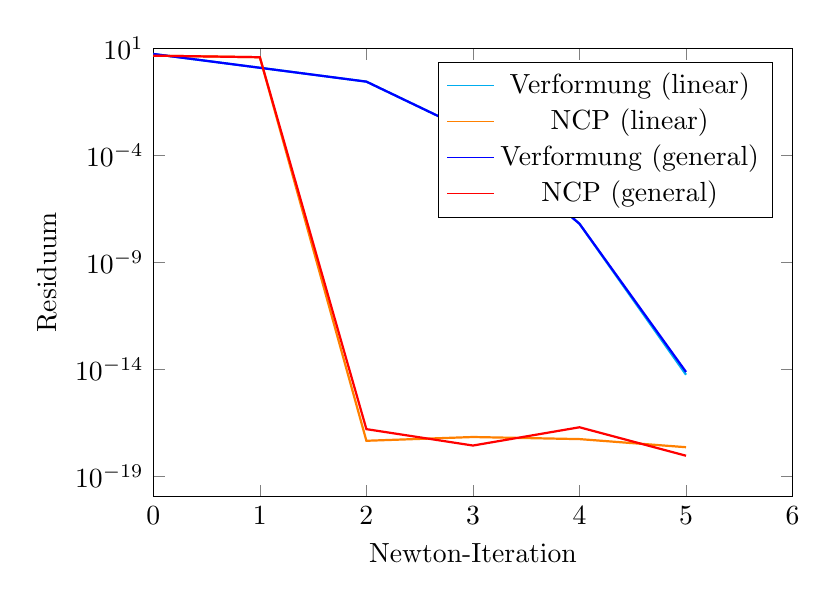
\begin{tikzpicture}[every plot/.append style={thick}] 
\begin{axis}[ 
label style={font=\normalsize}, 
xlabel={Newton-Iteration}, 
ylabel={Residuum}, 
xmin=0, xmax=6, 
ymode=log, 
ymin=0, ymax=10, 
width=0.8\textwidth, 
height=0.6\textwidth, 
legend pos=north east, 
legend style={cells={align=left}}, 
grid style=dashed, 
] 
\addplot[ 
color=cyan, 
] 
coordinates { 
(0, 5.35e+00)(1, 1.21e+00)(2, 2.72e-01)(3, 1.11e-03)(4, 6.12e-08)(5, 5.33e-15)}; 
\addlegendentry{Verformung (linear)} 
\addplot[ 
color=orange, 
] 
coordinates { 
(0, 4.46e+00)(1, 3.77e+00)(2, 4.34e-18)(3, 6.51e-18)(4, 5.20e-18)(5, 2.17e-18)}; 
\addlegendentry{NCP (linear)} 
\addplot[ 
color=blue, 
] 
coordinates { 
(0, 5.35e+00)(1, 1.21e+00)(2, 2.72e-01)(3, 1.11e-03)(4, 6.12e-08)(5, 7.18e-15)}; 
\addlegendentry{Verformung (general)} 
\addplot[ 
color=red, 
] 
coordinates { 
(0, 4.46e+00)(1, 3.77e+00)(2, 1.52e-17)(3, 2.60e-18)(4, 1.86e-17)(5, 8.67e-19)}; 
\addlegendentry{NCP (general)} 
\end{axis} 
\end{tikzpicture} 
\caption{Residuen des Stoffgesetzes 'Neo Hooke' mit Hinderniss 'Spitze' und 50 Freiheitsgraden für die Verschiebung.} 
\label{fiq:NeoHooke_Spitze_level1} 
\end{figure} 
